% !TeX root = ../../Book3.tex
\section{Abel 求和}
\label{b3:sec:2503}

前两节的约数恒等式都是有限的。进入无穷级数以前，还需要回答另一个问题：知道系数的部分和以后，怎样估计加了权重的和？例如，交错系数的单项大小始终为一，但前 \(N\) 项的和至多为一。若在估计中先把每项取绝对值，这种抵消就完全消失了。

本节把系数 \(a_n\) 与平滑权重 \(f(n)\) 分开处理。系数不必具有正性或连续性；需要掌握的是阶梯函数 \(A(x)=\sum_{n\le x}a_n\)。将加权和改写成含 \(A\) 的积分以后，抵消、平均主项和误差便都能保留下来。

\subsection{离散分部求和}
\label{b3:subsec:250301}

连续情形的分部积分把一个因子的导数转移到另一个因子上。有限求和也有同样的操作：把 \(a_n\) 写成部分和的差，再把差分转移到权重上。所得恒等式称为\term[abel-qiuhe]{Abel 求和}[Abel summation]。

\begin{proposition}[Abel 求和的有限形式]\label{b3:prop:25-summation-by-parts}
设 \(N\ge1\) 为整数，\(a_1,\ldots,a_N,b_1,\ldots,b_N\in\mathbb C\)，并令 \(A(0)=0\)、\(A(n)=\sum_{k=1}^n a_k\)。则
\[
 \sum_{n=1}^N a_nb_n
 =A(N)b_N+\sum_{n=1}^{N-1}A(n)(b_n-b_{n+1}).
\]
当 \(N=1\) 时，右侧第二个和按空和理解为零。
\end{proposition}
\begin{proof}
由 \(a_n=A(n)-A(n-1)\)，
\begin{align*}
 \sum_{n=1}^N a_nb_n
 &=\sum_{n=1}^N A(n)b_n-\sum_{n=1}^N A(n-1)b_n\\
 &=A(N)b_N+\sum_{n=1}^{N-1}A(n)b_n
                 -\sum_{n=0}^{N-1}A(n)b_{n+1}.
\end{align*}
最后一个和的 \(n=0\) 项为零，余下两和逐项合并就得到公式。
\end{proof}

公式中没有极限，也没有收敛假设。例如取 \(a_n=(-1)^{n-1}\)，则 \(A(n)\) 在奇数处为一、偶数处为零。若实权重满足 \(b_1\ge\cdots\ge b_N\ge0\)，右侧每个差 \(b_n-b_{n+1}\) 都非负，因而
\[
 \left|\sum_{n=1}^N(-1)^{n-1}b_n\right|
 \le b_N+\sum_{n=1}^{N-1}(b_n-b_{n+1})=b_1.
\]
直接对原和取绝对值只能得到 \(\sum b_n\)。Abel 求和的用途就在于先利用系数之间的抵消，再估计缓慢变化的权重。

\subsection{积分形式的部分求和}
\label{b3:subsec:250302}

若权重来自可微函数 \(f\)，有限差分 \(f(n)-f(n+1)\) 可写成导数的积分。

\begin{proposition}[Abel 求和的积分形式]\label{b3:prop:25-integral-summation}
设 \((a_n)_{n\ge1}\) 为复数列，\(x\ge1\) 为实数，\(f:[1,x]\to\mathbb C\) 连续可微，并对实数 \(t\ge1\) 置 \(A(t)=\sum_{n\le t}a_n\)。则
\begin{equation}\label{b3:eq:25-partial-summation}
 \sum_{n\le x}a_nf(n)
 =A(x)f(x)-\int_1^x A(t)f'(t)\,\mathrm dt.
\end{equation}
更一般地，若 \(1\le y\le x\)，只要求 \(f:[y,x]\to\mathbb C\) 连续可微，就有
\begin{equation}\label{b3:eq:25-interval-summation}
 \sum_{y<n\le x}a_nf(n)
 =A(x)f(x)-A(y)f(y)-\int_y^x A(t)f'(t)\,\mathrm dt.
\end{equation}
两式均包括整数端点和非整数端点。
\end{proposition}
\begin{proof}
先证第一式。令 \(N=\lfloor x\rfloor\)。在每个区间 \([n,n+1)\) 上，\(A(t)=A(n)\)，故
\[
 \int_1^x A(t)f'(t)\,\mathrm dt
 =\sum_{n=1}^{N-1}A(n)(f(n+1)-f(n))
    +A(N)(f(x)-f(N)).
\]
积分中有限个整数点的函数值不影响结果。代入 \(A(x)=A(N)\)，端点 \(A(x)f(x)\) 与最后一项合并为 \(A(N)f(N)\)，再用有限形式即可。当 \(x=N\) 时，最后一个积分区间长度为零，公式照常成立。

为证明第二式，可将 \(f\) 从 \([y,x]\) 连续可微地延到 \([1,x]\)：例如在 \(t\le y\) 时取 \(f(y)+f'(y)(t-y)\)。分别对上端 \(x\) 和 \(y\) 应用第一式，再相减；延拓部分的和与积分全部消去，得到所示区间公式。
\end{proof}

下端的开闭方式决定了补偿项。因为 \(A(y)\) 包含所有 \(n\le y\) 的项，\eqref{b3:eq:25-interval-summation}左侧求和必须是 \(y<n\le x\)。特别地，若 \(y\) 是整数，这个和不含 \(a_yf(y)\)；要改成闭区间，就应另加该项。检验 \(a_n=1,f=1\) 时，公式变为
\[
 \#\{n\in\mathbb N:y<n\le x\}=\lfloor x\rfloor-\lfloor y\rfloor,
\]
这也直接检查了整数端点的约定。

\subsection{加权和}
\label{b3:subsec:250303}

以后将系统研究复参数级数 \(\sum a_nn^{-s}\)。在本节先约定
\[
 t^{-s}=e^{-s\log t}\qquad(t>0,\ s\in\mathbb C),
\]
其中 \(\log t\) 是实对数，因而没有对数分支的选择。对实变量 \(t\) 求导得到 \((t^{-s})'=-s t^{-s-1}\)。应用\eqref{b3:eq:25-partial-summation}，便有有限恒等式
\[
 \sum_{n\le x}a_nn^{-s}
 =A(x)x^{-s}+s\int_1^x A(t)t^{-s-1}\,\mathrm dt.
\]
现在的问题是何时可以令 \(x\to\infty\)。这既要检查上端项，也要检查无穷积分。

\begin{proposition}[部分和增长与级数收敛]\label{b3:prop:25-partial-sum-convergence}
设 \((a_n)_{n\ge1}\) 为复数列，\(\alpha\in\mathbb R\)，并且存在常数 \(C\ge0\)，使
\[
 |A(x)|\le Cx^\alpha\qquad(x\ge1),
 \qquad A(x)=\sum_{n\le x}a_n.
\]
用实对数定义 \(n^{-s}=e^{-s\log n}\)。则级数 \(\sum_{n\ge1}a_nn^{-s}\) 在 \(\operatorname{Re}s>\alpha\) 收敛，其和在该半平面全纯，并且对每个实数 \(x\ge1\)、\(\sigma=\operatorname{Re}s>\alpha\)，
\begin{equation}\label{b3:eq:25-weighted-tail}
 \left|\sum_{n>x}a_nn^{-s}\right|
 \le C\left(1+\frac{|s|}{\sigma-\alpha}\right)x^{\alpha-\sigma}.
\end{equation}
这个收敛在半平面的每个紧子集上一致，且
\[
 \sum_{n\ge1}a_nn^{-s}
 =s\int_1^\infty A(t)t^{-s-1}\,\mathrm dt
 \qquad(\operatorname{Re}s>\alpha).
\]
\end{proposition}
\begin{proof}
固定 \(s\)，记 \(\sigma=\operatorname{Re}s>\alpha\)。上端项满足
\[
 |A(x)x^{-s}|\le Cx^{\alpha-\sigma}\longrightarrow0,
\]
而积分绝对值有界于
\[
 C\int_1^\infty t^{\alpha-\sigma-1}\,\mathrm dt
 =\frac C{\sigma-\alpha}<\infty.
\]
因此有限恒等式的右侧有极限，原级数就收敛，并有命题中的积分表示。这一步没有把 \(\sum|a_n|n^{-\sigma}\) 作为已知的收敛级数。

从积分表示中减去到 \(x\) 为止的有限恒等式，得
\[
 \sum_{n>x}a_nn^{-s}
 =-A(x)x^{-s}+s\int_x^\infty A(t)t^{-s-1}\,\mathrm dt.
\]
对两项分别取绝对值，利用
\(\int_x^\infty t^{\alpha-\sigma-1}\,\mathrm dt
 =x^{\alpha-\sigma}/(\sigma-\alpha)\)，就得到\eqref{b3:eq:25-weighted-tail}。

若 \(K\subset\{\operatorname{Re}s>\alpha\}\) 为紧集，则可取 \(\delta>0,R<\infty\)，使 \(s\in K\) 时 \(\operatorname{Re}s-\alpha\ge\delta\)、\(|s|\le R\)。上界于是统一为 \(C(1+R/\delta)x^{-\delta}\)，趋于零。每个有限部分和都是整函数，局部一致极限的全纯性给出最后的结论。
\end{proof}

通常只写 \(A(x)=O(x^\alpha)\)，即上述不等式最初只对充分大的 \(x\) 成立。由于任意有界区间内只有有限个系数，扩大 \(C\) 就能使它对所有 \(x\ge1\) 成立。尾界中的分母 \(\sigma-\alpha\) 说明了离边界的距离为什么重要；该估计不能直接用到 \(\sigma=\alpha\)。因子 \(|s|\) 则来自权重的导数，它也说明紧集上一致收敛不等于在整条无界竖线上有同一个常数。

对 \(a_n=(-1)^{n-1}\)，有 \(|A(x)|\le1\)，故 \(\sum(-1)^{n-1}n^{-s}\) 在 \(\operatorname{Re}s>0\) 局部一致收敛。但其绝对值级数为 \(\sum n^{-\sigma}\)，在 \(0<\sigma\le1\) 发散。到了边界 \(\sigma=0\)，原级数的单项绝对值恒为一，也不可能收敛。这个例子同时显示了抵消带来的好处和增长估计的边界。

部分和不只是给出一个增长界。有时还知道它由平均主项与较小误差组成，此时主项会在变换中留下一个极点。
\begin{proposition}[平均主项与解析奇部]\label{b3:prop:25-mean-pole}
设 \((a_n)_{n\ge1}\) 为复数列，\(c\in\mathbb C\)、\(0\le\beta<1\)，并且当实数 \(x\to\infty\) 时，
\[
 A(x)=\sum_{n\le x}a_n=cx+O(x^\beta).
\]
用实对数定义 \(n^{-s}=e^{-s\log n}\)。则级数 \(D_a(s)=\sum_{n\ge1}a_nn^{-s}\) 在 \(\operatorname{Re}s>1\) 收敛，并有亚纯延拓
\[
 D_a(s)=\frac{cs}{s-1}+s\int_1^\infty(A(t)-ct)t^{-s-1}\,\mathrm{d}t,
 \qquad \operatorname{Re}s>\beta,
\]
其中右端在 \(s=1\) 处按亚纯函数理解。它在该半平面除 \(s=1\) 的可能单极点外全纯，该点留数为 \(c\)；当 \(c=0\) 时，该点也全纯。
\end{proposition}
\begin{proof}
假设首先给出 \(A(x)=O(x)\)，所以\cref{b3:prop:25-partial-sum-convergence}保证在 \(\operatorname{Re}s>1\) 时，
\[
 D_a(s)=s\int_1^\infty A(t)t^{-s-1}\,\mathrm dt.
\]
在这一半平面里，把 \(A(t)\) 分成 \(ct+E(t)\)，其中 \(E(t)=A(t)-ct=O(t^\beta)\)。主项的积分为
\[
 cs\int_1^\infty t^{-s}\,\mathrm dt=\frac{cs}{s-1}.
\]
误差积分在 \(\operatorname{Re}s>\beta\) 已经绝对收敛。若参数限制在紧集 \(K\) 中，取 \(\delta>0\) 使 \(\operatorname{Re}s\ge\beta+\delta\)，则被积函数由常数倍 \(t^{-1-\delta}\) 控制。对参数求导只增加一个 \(\log t\)，而 \(t^{-1-\delta}\log t\) 仍可积。因此可以对误差积分作参数微分，它在较大的半平面全纯。

右端与原级数在 \(\operatorname{Re}s>1\) 相等，故构成所说的延拓。由于 \(\beta<1\)，误差积分在一的某个邻域全纯；又 \(cs/(s-1)=c+c/(s-1)\)，留数恰为 \(c\)。
\end{proof}

例如，若 \(a_n\) 的周期为正整数 \(q\)，令 \(c=q^{-1}\sum_{r=1}^q a_r\)。将 \(\lfloor x\rfloor\) 写成若干整周期与不足 \(q\) 项的余段，整周期总和为周期数乘 \(qc\)，余段的和有界；再用 \(x-\lfloor x\rfloor<1\)，便得 \(A(x)=cx+O(1)\)。于是相应级数的和可亚纯延拓到 \(\operatorname{Re}s>0\)。若 \(c=0\)，部分和本身有界，原级数就已在这个半平面收敛，且极点消失；交错系数是其中最简单的例子。

若 \(c\ne0\)，较大的延拓域却不能直接说成原级数的收敛域。取 \(a_n=1\) 时，下面的公式将给出 \(0<s<1\) 上有限的延拓值，而正项级数 \(\sum n^{-s}\) 在这些实数点发散。延拓保留了原函数的解析关系，但其新值不必由原求和过程给出。

还要区别另一个方向：从 \(A(x)=cx+O(x^\beta)\) 推出变换的极点，并不等于从一个极点就能恢复 \(A(x)\sim cx\)。上面的证明将已知的误差界放进积分；逆向则要由变换控制未知的部分和。后面的 Tauber 型定理会为这种逆向推断补充条件。


\subsection{积分比较与除数函数的平均值}
\label{b3:subsec:250304}

先看最简单的系数 \(a_n=1\)。此时 \(A(t)=\lfloor t\rfloor=t-\{t\}\)，其中分数部分 \(\{t\}=t-\lfloor t\rfloor\in[0,1)\)。由刚才的积分表示，当 \(\operatorname{Re}s>1\) 时，
\begin{equation}\label{b3:eq:25-zeta-integral}
\sum_{n\ge1}n^{-s}=\frac{s}{s-1}-s\int_1^\infty\{t\}t^{-s-1}\,\mathrm{d}t.
\end{equation}
右端的积分在 \(\operatorname{Re}s>0\) 全纯，因为分数部分有界。它在 \(s=1\) 附近没有奇性，整个表达式在一的留数为一。下一章将从这里继续研究 \(\zeta\) 函数的延拓；目前只需要注意，公式左端作为级数的等号先在 \(\operatorname{Re}s>1\) 成立。

在实参数 \(s=1\) 处，原级数发散，不能直接用这条无穷求和公式计算有限部分和。记 \(H_N=\sum_{n=1}^N1/n\)。\cref{b3:prop:21-euler-constant}已经证明 Euler 常数 \(\gamma=\lim_{N\to\infty}(H_N-\log N)\) 存在，并给出更精细的截断误差；此处只需恢复
\[
 H_N=\log N+\gamma+O(N^{-1})\qquad(N\ge1).
\]
这个 \(O(N^{-1})\) 不能随意换成较粗的 \(O(1)\)，因为下面它将与一个大的参数相乘。其大小也可从相邻差重新看出：
\[
 0\le (H_N-\log N)-(H_{N+1}-\log(N+1))
 \le\frac1N-\frac1{N+1}.
\]
将此不等式从 \(N\) 到无穷求和，便得 \(0\le H_N-\log N-\gamma\le1/N\)。

现在考虑约数个数 \(d(n)=\#\{a\in\mathbb N:a\mid n\}\)。每个约数 \(a\mid n\) 唯一决定配对因子 \(b=n/a\)，所以累积和 \(\sum_{n\le x}d(n)\) 正好计数正整数点 \(ab\le x\)。单个 \(d(n)\) 会随着素因子结构起伏，而这个几何计数更容易得到平滑主项。

\begin{proposition}[除数个数的平均值]
\label{b3:prop:25-divisor-average}
设 \(d(n)\) 为正整数 \(n\) 的正约数个数，以 \(\gamma\) 表示 Euler 常数，即
\[
 \gamma=\lim_{N\to\infty}\left(\sum_{n=1}^N\frac1n-\log N\right).
\]
则当实数 \(x\to\infty\) 时，
\[
 \sum_{n\le x}d(n)=x\log x+(2\gamma-1)x+O(\sqrt x).
\]
其中误差估计可用一个与 \(x\ge2\) 无关的常数。
\end{proposition}
\begin{proof}
将计数记为 \(D(x)=\sum_{n\le x}d(n)\)，令 \(y=\lfloor\sqrt x\rfloor\)。每个满足 \(ab\le x\) 的正整数点至少有一个坐标不超过 \(y\)，否则 \(a,b\ge y+1\)，从而 \(ab\ge(y+1)^2>x\)。

先数 \(a\le y\) 的点。固定 \(a\) 后，\(b\) 可以取 \(1,\ldots,\lfloor x/a\rfloor\)，故点数为 \(\sum_{a\le y}\lfloor x/a\rfloor\)。交换两个坐标，\(b\le y\) 的点数也相同。这两部分的交集恰是 \(1\le a,b\le y\) 的整个整数方块，因为 \(ab\le y^2\le x\)。它有 \(y^2\) 个点，被重复计算了一次，应减去一次。因此
\begin{equation}\label{b3:eq:25-hyperbola-count}
 D(x)=2\sum_{a\le y}\left\lfloor\frac xa\right\rfloor-y^2.
\end{equation}
这是有限计数恒等式，尚未作任何近似。

每个取整值与原数相差小于一，而现在只剩 \(y\) 项，故
\[
 D(x)=2xH_y-y^2+O(y)
     =2x\log y+2\gamma x-y^2+O(x/y+y).
\]
对 \(x\ge4\)，有 \(y=\sqrt x+O(1)\) 且 \(y\ge\sqrt x/2\)。于是
\[
 2\log y=\log x+O(x^{-1/2}),\qquad
 y^2=x+O(\sqrt x),\qquad x/y+y=O(\sqrt x).
\]
将这些估计逐项代入，得到所求公式；在有界区间 \(2\le x<4\) 上扩大误差常数即可。
\end{proof}

\cref{b3:fig:25-hyperbola}将 \(x=12\)、\(y=3\) 的分割画出。左侧三列各有 \(12,6,4\) 个点，下侧三行也一样，中间 \(3\times3\) 的九个点被数了两次。因此 \(D(12)=2(12+6+4)-9=35\)。正整数点若同时落在这两条带以外，两个坐标至少为四，乘积已经大于十二。

\begin{figure}[htbp]
\centering
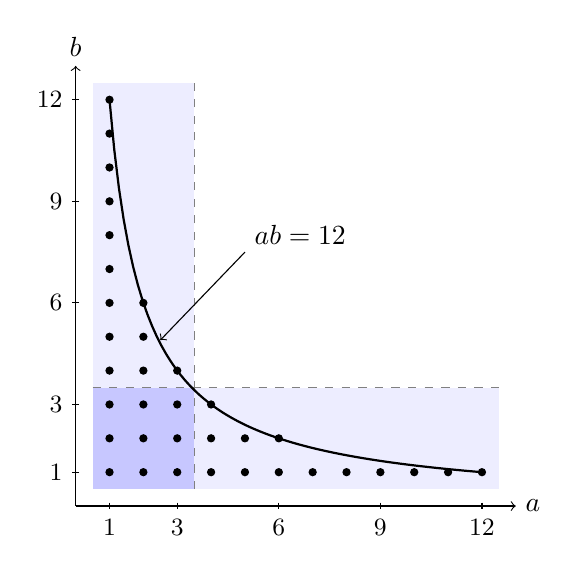
\begin{tikzpicture}[x=0.43cm,y=0.43cm]
 \fill[blue!7] (0.5,0.5) rectangle (3.5,12.5);
 \fill[blue!7] (0.5,0.5) rectangle (12.5,3.5);
 \fill[blue!22] (0.5,0.5) rectangle (3.5,3.5);
 \draw[->] (0,0) -- (13,0) node[right] {\(a\)};
 \draw[->] (0,0) -- (0,13) node[above] {\(b\)};
 \draw[dashed,gray] (3.5,0.5) -- (3.5,12.5);
 \draw[dashed,gray] (0.5,3.5) -- (12.5,3.5);
 \draw[thick,domain=1:12,samples=80] plot (\x,{12/\x});
 \foreach \a in {1,...,12} {
  \foreach \b in {1,...,12} {
   \pgfmathtruncatemacro{\within}{\a*\b<=12}
   \ifnum\within=1\relax
    \fill (\a,\b) circle (1.5pt);
   \fi
  }
 }
 \foreach \t in {1,3,6,9,12} {
  \draw (\t,0.10) -- (\t,-0.10) node[below,font=\small] {\(\t\)};
  \draw (0.10,\t) -- (-0.10,\t) node[left,font=\small] {\(\t\)};
 }
 \node[anchor=west] at (5,8) {\(ab=12\)};
 \draw[->] (5,7.5) -- (2.5,4.9);
\end{tikzpicture}
\caption{双曲线分割：圆点为 \(ab\le12\) 的正整数点。两条浅色带分别选出 \(a\le3\) 与 \(b\le3\) 的整数坐标；深色方块中的九个点需减去一次。}
\label{b3:fig:25-hyperbola}
\end{figure}

这种利用双曲线两侧对称计数的办法称为\term[dirichlet-shuangquxian-fa]{Dirichlet 双曲线法}[Dirichlet hyperbola method]。若直接把 \(\sum_{a\le x}\lfloor x/a\rfloor\) 中每项替成 \(x/a\)，会累积 \(O(x)\) 的取整误差，因而看不见线性次项。以 \(\sqrt x\) 分割以后，只需近似约 \(\sqrt x\) 项，误差便缩小到平方根尺度。若在一个很小的阈值处分割，另一方向仍会留下很长的和；平方根使两个方向的长度保持同一数量级。

部分求和还能把已有的平均值换成新的权重。由刚才的结果，置 \(c=2\gamma-1\)，可写 \(D(t)=t\log t+ct+E(t)\)，其中 \(E(t)=O(\sqrt t)\) 对所有 \(t\ge1\) 成立。取权重 \(1/n\)，得到
\begin{align*}
 \sum_{n\le x}\frac{d(n)}n
 &=\frac{D(x)}x+\int_1^x\frac{D(t)}{t^2}\,\mathrm dt\\
 &=\log x+c+\frac12(\log x)^2+c\log x+O(1)\\
 &=\frac12(\log x)^2+2\gamma\log x+O(1).
\end{align*}
这里端点的误差 \(E(x)/x=O(x^{-1/2})\) 有界，误差积分也一致有界，因为
\[
 \int_1^\infty\frac{|E(t)|}{t^2}\,\mathrm dt
 \le C\int_1^\infty t^{-3/2}\,\mathrm dt<\infty.
\]
一次计数所得的主项与误差，就这样转变成了另一个加权平均值；不需要重新逐项估计 \(d(n)\)。

\subsection{素数计数函数的应用}
\label{b3:subsec:250305}

素数的分布没有简单的逐项公式，但部分求和仍然适用。对实数 \(x\ge2\)，记
\[
 \pi(x)=\#\{p\le x:p\text{ 为素数}\},\qquad
 \vartheta(x)=\sum_{p\le x}\log p.
\]
函数 \(\pi\) 称为\term[sushu-jishu-hanshu]{素数计数函数}[prime-counting function]；函数 \(\vartheta\) 给每个素数加上对数权重。这里的 \(\pi(x)\) 是函数记号，与圆周率 \(\pi\) 应依上下文区分。

在\eqref{b3:eq:25-interval-summation}中取 \(y=2\)，令 \(a_n\) 在素数处为一、其余处为零，并取 \(f(t)=\log t\)。左端不含素数二，故
\[
 \vartheta(x)-\log2
 =\pi(x)\log x-\pi(2)\log2-\int_2^x\frac{\pi(t)}t\,\mathrm dt.
\]
因为 \(\pi(2)=1\)，两个下端项抵消，得到
\begin{equation}\label{b3:eq:25-prime-log-weight}
 \vartheta(x)=\pi(x)\log x-\int_2^x\frac{\pi(t)}t\,\mathrm dt
 \qquad(x\ge2).
\end{equation}
反过来，令 \(a_n\) 在素数处为 \(\log n\)、其余处为零，取 \(f(t)=1/\log t\)。这个权重在 \([2,x]\) 上连续可微，不涉及 \(t=1\) 的奇性。区间公式给
\[
 \pi(x)-1
 =\frac{\vartheta(x)}{\log x}-\frac{\vartheta(2)}{\log2}
       +\int_2^x\frac{\vartheta(t)}{t(\log t)^2}\,\mathrm dt.
\]
利用 \(\vartheta(2)=\log2\)，得到
\begin{equation}\label{b3:eq:25-prime-remove-weight}
 \pi(x)=\frac{\vartheta(x)}{\log x}
       +\int_2^x\frac{\vartheta(t)}{t(\log t)^2}\,\mathrm dt
 \qquad(x\ge2).
\end{equation}
两式在 \(x=2\) 时也成立，此时积分均为零。

\begin{proposition}[素数计数的两种渐近形式]\label{b3:prop:25-prime-counting-equivalence}
对实数 \(x\ge2\)，令 \(\pi(x)=\#\{p\le x:p\text{ 为素数}\}\)、\(\vartheta(x)=\sum_{p\le x}\log p\)。则当 \(x\to\infty\) 时，以下两项等价：
\[
 \vartheta(x)\sim x,\qquad \pi(x)\sim\frac{x}{\log x}.
\]
\end{proposition}
\begin{proof}
先假设 \(\vartheta(x)\sim x\)。这蕴含存在常数 \(C\)，使 \(0\le\vartheta(t)\le Ct\) 对所有 \(t\ge2\) 成立。对 \(x\ge4\)，将\eqref{b3:eq:25-prime-remove-weight}中的积分在 \(\sqrt x\) 处分开：
\begin{align*}
 0\le\int_2^x\frac{\vartheta(t)}{t(\log t)^2}\,\mathrm dt
 &\le C\int_2^{\sqrt x}\frac{\mathrm dt}{(\log t)^2}
       +C\int_{\sqrt x}^x\frac{\mathrm dt}{(\log t)^2}\\
 &\le\frac{C\sqrt x}{(\log2)^2}
       +\frac{4Cx}{(\log x)^2}
 =o\left(\frac x{\log x}\right).
\end{align*}
第一段虽不使用对数衰减，但长度只有 \(\sqrt x\)；第二段长度较大，整个区间上的对数却至少为 \(\frac12\log x\)。因此积分是低阶项，端点项 \(\vartheta(x)/\log x\sim x/\log x\) 给出所求渐近。

反过来，假设 \(\pi(x)\sim x/\log x\)。扩大常数以后，\(0\le\pi(t)\le Ct/\log t\) 对所有 \(t\ge2\) 成立。同样分割可得
\[
 0\le\int_2^x\frac{\pi(t)}t\,\mathrm dt
 \le\frac{C\sqrt x}{\log2}+\frac{2Cx}{\log x}=o(x).
\]
代入\eqref{b3:eq:25-prime-log-weight}，再用 \(\pi(x)\log x\sim x\)，便得到 \(\vartheta(x)\sim x\)。
\end{proof}

这个命题把两种计数的渐近联系起来：建立其中一种以后，Abel 求和便给出另一种。后文由 \(\zeta\) 函数的解析性质研究素数时，对数权重更自然地出现，因此会先估计带权部分和，再用这里的公式还原为素数个数。
